A continuación se tratará con más detalle el sistema de generación de personajes, que es un componente clave 
para la creación de mundos dinámicos y brindar la aparencia de un mundo con vida. Este sistema se podría 
categorizar en dos tipos principales: los jugadores (\textit{players}) y los \textit{NPCs} 
(\textit{Non-Playable Character}). Los jugadores son los personajes controlados por los usuarios, 
mientras que los \textit{NPCs} son personajes que son diseñados por los creadores de mundos.

Dentro de los \textit{NPCs} se encuentran dos subtipos principales: los \textit{NPCs} pasivos y los \textit{NPCs} 
agresivos o enemigos.

Los \textit{NPCs} pasivos con los que el jugador puede interactuar mediante diálogos. Mientras que 
los \textit{NPCs} agresivos son personajes hostiles que atacan al jugador.

\vspace{0.15cm}

Para un creador de mundos, es esencial poder colocar \textit{NPCs} en su mundo para que el personaje pueda 
interactuar con ellas. Sumado a esto, es importante que el creador pueda configurar sus aparencias para 
poder crear un mundo con una ambientación específica, y darle personalidad a su mundo. 

Para esto, se han implementado funcionalidades de personalización de personajes, que permiten a los 
creadores configurar la apariencia de todos los \textit{NPCs}, pudiendo elegir entre distintas opciones de 
ropa, accesorios y colores para cada parte del cuerpo.

\vspace{0.25cm}

A continuación se muestra una captura de pantalla del editor de mundos para la creación los \textit{NPCs} 
pasivos. En ellos se pueden configurar sus diálogos, su apariencia, y también se les puede asignar 
misiones. Se verá a mas detalle en su sección a parte más adelante.


\begin{figure}[H]
  \centering
  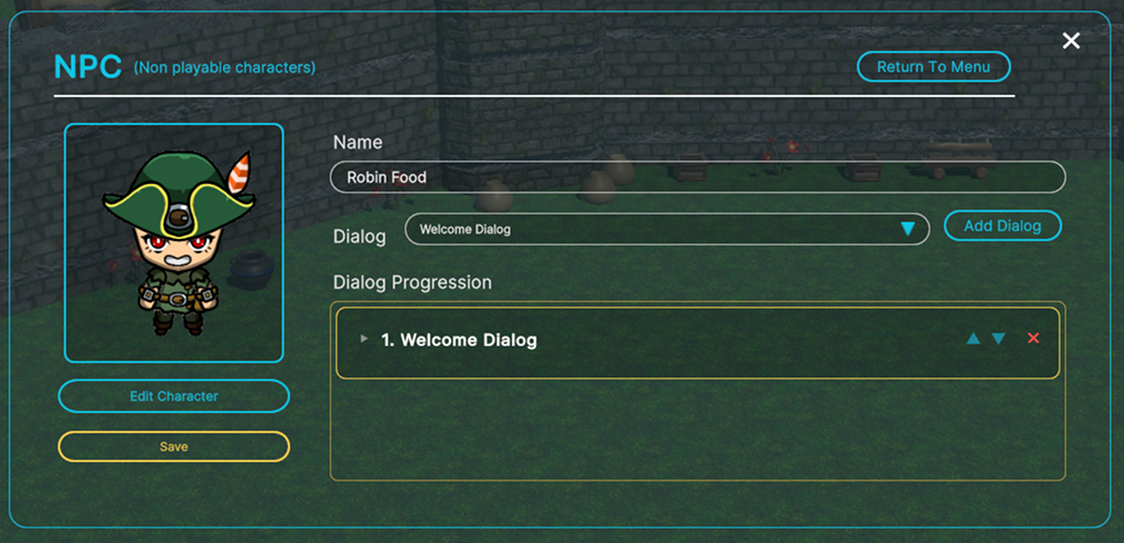
\includegraphics[width=1\textwidth]{img/08-implemented-solution/product/npc-creation.jpg}
  \caption{Todos los tipos de generadores colocado en la escena.}
\end{figure}


Luego se muestra una captura de pantalla del editor de mundos para la creación de los \textit{NPCs} agresivos, 
o enemigos. En el caso de los \textit{NPCs} agresivos, se les puede asignar un arma específica, lo que afecta 
su comportamiento de ataque y su dificultad. La estadística del arma está ligada a la dificultad del enemigo, 
por lo que un enemigo con un arma de mayor daño será más difícil de derrotar. Esto permite a los 
creadores, si lo desean, diseñar enemigos con diferentes niveles de dificultad, y crear una experiencia de juego 
más variada, progresiva y desafiante para los jugadores. También, como se nombró en secciones anteriores, a los 
enemigos se les puede asignar una tabla de botín que se recompensan al ser derrotados.

\vspace{0.25cm}

Por último, como carácteristica de personalización del mundo, se ha diseñado un sistema de generación de 
personajes, que permite a los creadores colocar generadores dentro de su mundo. Los 
\textbf{Generadores (\textit{Spawners})}, que son objetos que crean personajes en tiempo de ejecución y 
pueden configurarse con parámetros como frecuencia de aparición, rango y tipo de entidad a generar. 
Actualmente, se encuentran disponibles tres tipos: generador de enemigos (\textit{Enemy Spawner}), 
generador de \textit{NPCs} (\textit{NPC Spawner}) y generador de jugadores (\textit{Player Spawner}).

\begin{figure}[H]
  \centering
  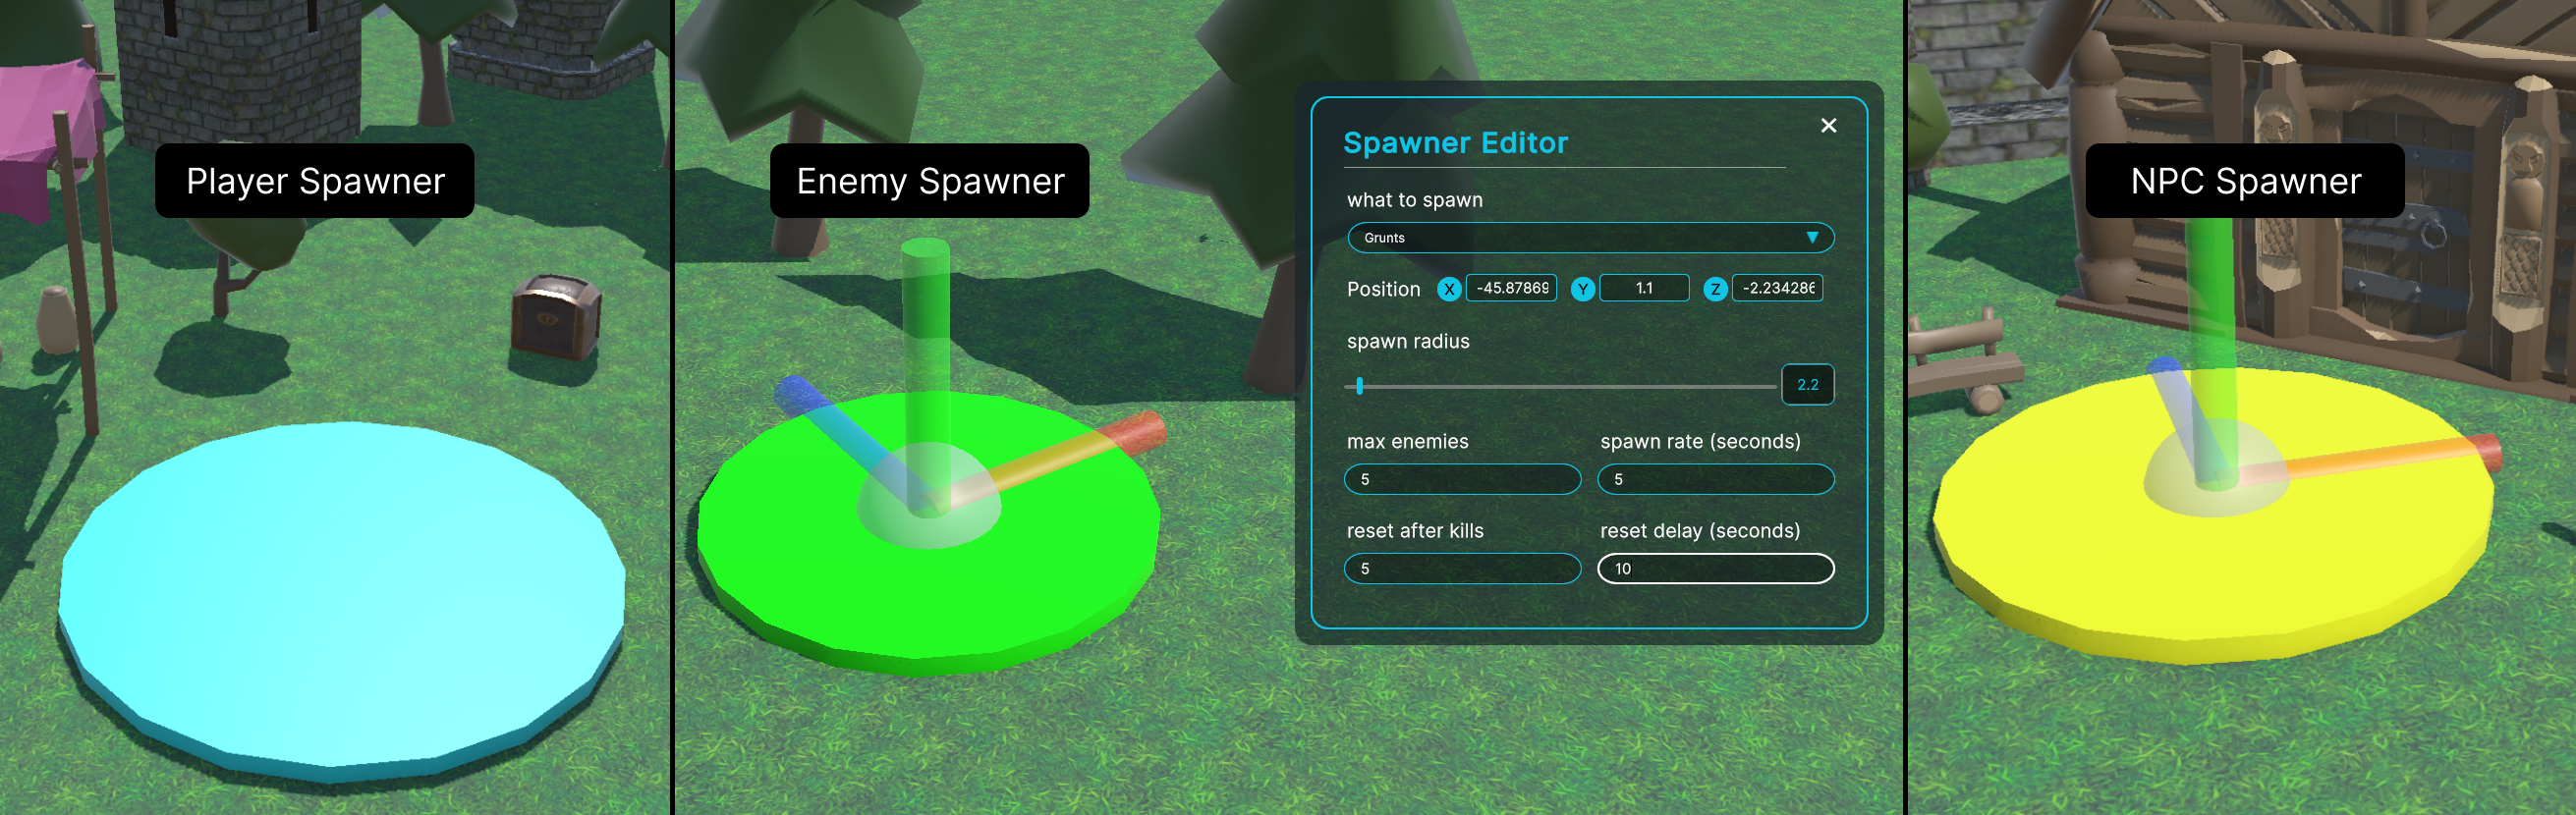
\includegraphics[width=\textwidth]{img/08-implemented-solution/product/spawners.jpg}
  \caption{Todos los tipos de generadores colocado en la escena.}
\end{figure}